\documentclass[11pt]{article}

\usepackage[letterpaper,margin=1in]{geometry}
\usepackage{amsmath,amssymb}
\usepackage{booktabs}
\usepackage{microtype}
\usepackage{times}
\usepackage[T1]{fontenc}
\usepackage[utf8]{inputenc}
\usepackage{titlesec}
\usepackage{enumitem}
\usepackage[hidelinks]{hyperref}
\usepackage{url}
\Urlmuskip=0mu plus 1mu\relax
\usepackage{xcolor}
\usepackage{array}
\usepackage{graphicx}
\graphicspath{{figs/}}

\titleformat{\section}{\normalfont\large\bfseries}{\thesection}{0.6em}{}
\setlength{\parskip}{0.4em}
\setlength{\parindent}{0pt}
\renewcommand{\arraystretch}{1.15}

\title{\textbf{Witnesses, Not Amplifiers:\\ What Specialist Agents Contribute to
Epistemic Quality}}
\author{Sam Bobo}
\date{Draft v0.1 --- August 2026 \quad$\vert$\quad Target: arXiv cs.CL}

\begin{document}
\sloppy
\maketitle

\begin{abstract}
\noindent
Multi-agent pipelines are often built on the premise that specialist models
bring better judgement to their domains, and that an aggregator's job is to
preserve it. We tested that premise directly and found both halves wrong. A
domain-specialised medical model, asked a question under a neutral prompt,
qualifies its claims no more than a generic model of similar size---$0.15$
against $0.14$. Its apparent richness inside a pipeline comes entirely from
the instruction in its system prompt. And a single well-prompted model
matches an entire three-specialist council for sheer quantity of qualification
($0.50$ against $0.57$, overlapping intervals). On this measure, specialists
contribute nothing that an instruction does not.

Worse, tuning them upward is actively harmful. Prompting or fine-tuning a
specialist to qualify more than doubles what it writes, and the finished
answer gets \emph{worse}---$1.21$ untrained against $0.92$ for both methods.
Extending the treatment to more specialists makes it worse monotonically
($\rho = -0.80$). The aggregator does not preserve what arrives; it decides
afresh, and reads saturated hedging as noise to be edited out. What
specialists actually contribute is narrower and more useful: \emph{grounds}
for a conditional instruction. The council was the only arrangement we tested
that qualified heavily where warranted and not at all where it was not
($0.00$ $[0.00,0.00]$ against a lone prompted model's $0.15$ $[0.08,0.22]$),
because its final instruction can check what the specialists flagged. A
solitary model has nothing to check. Specialists are worth their cost as
witnesses, not as amplifiers---and the practical consequence is that effort
spent making them more careful is worse than wasted, while effort spent on
the aggregator's instruction is the only thing that pays.
\end{abstract}

\begin{center}
\fbox{\begin{minipage}{0.93\linewidth}\small
\textbf{Correction (August 2026).} Claims in this draft that the council
achieves better \emph{calibration} than a single prompted model---that it
qualifies substantially where warranted and not at all where it is not---are
\textbf{withdrawn}. They rested on a trigger-free question that is off-topic
for the specialists, on which the planner routes to nobody and the pipeline
bypasses the conditional instruction; the reported $0.00$ came from a prompt
containing no preservation clauses. A controlled retest on trigger-free
questions the planner does engage with gives the council $0.64$ $[0.36,0.95]$
against a lone prompted model's $0.31$ $[0.21,0.42]$. Results concerning
volume, the instruction mechanism, the training nulls, and the specialists'
contribution are unaffected.
\end{minipage}}
\end{center}

\begin{center}
\fbox{\begin{minipage}{0.93\linewidth}\small
\textbf{Correction (August 2026), continued.} The claim that the models share
a common \emph{intrinsic band} under a neutral prompt is weakened: for three of
the four, $70$--$80\%$ of runs contain no epistemic marker at all, so the
matching densities reflect a floor rather than a shared level, and per-character
normalization coincidentally equates a model that emits $3.3\times$ more
markers in $3.7\times$ more text. The supportable statement is that these
models produce \emph{almost none} unprompted and cannot be distinguished there.
The contrast that carries the argument---the same specialist model at zero
markers in $80\%$ of neutral runs versus $1.31$ as an instructed pipeline
seat---is unaffected, being within-model and spanning the floor.
\end{minipage}}
\end{center}

\section{Introduction}
The case for multi-agent pipelines usually rests on division of labour: a
medical model should reason better about medicine, a legal model about law,
and an aggregator should combine their contributions without losing what makes
each valuable. Where the valuable thing is epistemic---a flagged assumption, a
noted uncertainty, a caveat about currency of information---the same case
implies two things. Specialists should be better at producing it, and the
aggregator's job is to preserve it.

We set out to strengthen a pipeline along exactly those lines and could not.
This paper reports what we found instead, in the order that makes the argument
rather than the order we found it.

Neither premise survives contact with a control. Specialisation does not
produce epistemic care: a domain-tuned medical model and a generic model of
similar size, given the same neutral prompt, qualify their claims at
indistinguishable rates. The specialist looks careful inside a pipeline only
because its system prompt tells it to be. And quantity of care does not require
specialists at all---one model with a good instruction matches a full council.

The second premise fails harder, and in the opposite direction from the
obvious failure mode. Making specialists more careful does not merely fail to
help; it makes the finished answer worse, reliably, by two different methods
and monotonically in the number of specialists treated. An aggregator does not
carry qualification through. It decides how much to write, largely
independently of how much it received, and past a point additional input
suppresses rather than adds.

What remains is a narrower role, and we think a correct one. A specialist's
contribution is not volume but \emph{evidence}: a record of what was flagged,
against which the aggregator's instruction can be made conditional. That
distinction is what separates the council from a lone prompted model. The two
match on how much they qualify; they differ completely on whether they qualify
when nothing warrants it. One can check what its specialists said. The other
is guessing.

We call this the difference between a witness and an amplifier, and the rest
of the paper is the evidence for it.

\section{Setup}
\textbf{Pipeline.} Four models running locally on one 32\,GB machine: a
planner/aggregator (Phi-4-14B unless stated) and three domain specialists
(Llama3-Med42-8B, Saul-7B-Instruct, Qwen-Open-Finance-8B), all quantised. The
planner decomposes a question and sends each specialist a self-contained
sub-question; specialists never see the original query. The aggregator then
writes the final answer under an instruction that asks it to surface
disagreements and to preserve specific things the specialists flagged. The
full instruction is in Appendix~\ref{app:prompt}.

\textbf{What we measure.} We count four families of epistemic behavior per
1{,}000 characters: disclosing that information may post-date training,
labelling a number as an assumption, distinguishing jurisdictions or regimes,
and calibrated hedging. A fifth---distinguishing near-synonymous terms of
art---fell below detection and is dropped. Counting is done by pattern
matching, cross-checked on the load-bearing comparisons by a calibrated
entailment model and by blinded pairwise LLM judges shown both texts in each
order (Appendix~\ref{app:instr}).

\textbf{Questions.} Seven cases spanning healthcare, law and finance. Six
warrant qualification: they turn on guidance that may have changed, on
quantities the question leaves unstated, or on conflicting jurisdictions. The
seventh deliberately warrants none---every figure it needs is given and
nothing in it has moved in a decade. That case does most of the work in this
paper, because a system that qualifies everything is otherwise
indistinguishable from one that qualifies the right things.

\textbf{Scale.} Roughly 1{,}300 runs, five seeds per condition, intervals by
bootstrap. Predictions were registered before the runs that test them, and
we report the ones that failed.

\section{Specialisation does not produce epistemic care}
The first premise is testable in isolation. Take the specialists out of the
pipeline, give them a neutral instruction---answer the question directly and
substantively---and see whether they qualify more than a generic model.

They do not. Med42-8B, a Llama-3 model tuned on clinical data and preference-
aligned, produces $0.15$ $[0.04,0.28]$. Mistral-7B-Instruct produces $0.14$
$[0.04,0.26]$; Qwen2.5-7B-Instruct $0.14$ $[0.06,0.24]$; a 20B mixture-of-
experts, measured the same way, $0.14$. Four models on four different
architectures, spanning clinical fine-tuning and generic instruction tuning,
all sit within $0.01$ of each other.

The same model, placed in the pipeline as a specialist, produces $1.31$
$[1.02,1.63]$---nearly nine times more, with intervals nowhere near
overlapping. Nothing about the model changed. What changed is that its system
prompt in the pipeline says \emph{``Flags training-cutoff uncertainty
EXPLICITLY when guidelines or evidence may have evolved,''} and that the
planner appends a further reminder to do so when it judges the question
time-sensitive---which it did in 30 of 34 runs.

So the specialist's epistemic richness is an instruction, not an expertise.
This is worth stating plainly because it is the premise on which specialist
pipelines are usually justified, and because it is cheap to check and, as far
as we can tell, rarely checked.

\section{Nor do specialists supply quantity}
If specialists do not produce care by being specialists, perhaps they produce
it by being many. We tested this by holding the model fixed---the same 20B
model in every role---and varying only the shape of the arrangement across six
designs, so that any difference is attributable to structure alone
(Fig.~\ref{fig:arch}).

\begin{figure}[t]
\centering
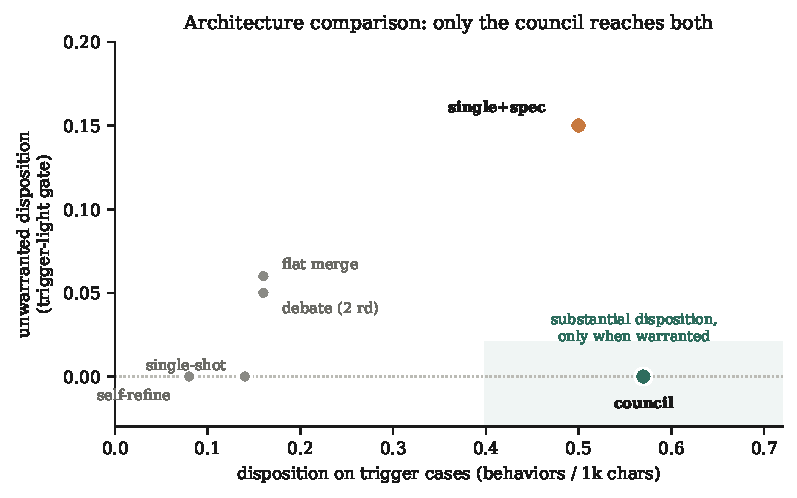
\includegraphics[width=0.80\linewidth]{fig_arch.pdf}
\caption{Six arrangements, one model in every role (210 runs). Horizontal:
qualification where it is warranted. Vertical: qualification where it is
\emph{not}. Three specialists merged plainly, and two rounds of debate, barely
leave the single-model corner. A lone prompted model reaches full volume but
qualifies a question that warrants nothing. Only the council reaches the
shaded region.}
\label{fig:arch}
\end{figure}

Three specialists whose answers are merged with a plain instruction reach
$0.16$ $[0.11,0.22]$---indistinguishable from one model answering alone at
$0.14$ $[0.09,0.19]$. Two full rounds of debate, in which each specialist
revises after reading the others, reach $0.16$ $[0.12,0.20]$: more
deliberation, no more care. A single model asked to draft, critique itself and
revise reaches $0.08$, the lowest of any arrangement---self-criticism tightens
prose and the qualifications are the first thing to go.

Meanwhile a single model given a good instruction and no specialists at all
reaches $0.50$ $[0.41,0.60]$, against the full council's $0.57$
$[0.45,0.71]$. The intervals overlap. On quantity of qualification, three
specialists and a planner buy nothing over one model and a paragraph of
instruction.

\section{Tuning specialists upward makes the answer worse}
The remaining hope for the standard picture is that specialists are simply
under-tuned---that a specialist trained to qualify more would push more
through. We tested this at the specialist in three ways, and it fails in a way
that is more informative than a null (Fig.~\ref{fig:witness}, left).

\begin{figure}[t]
\centering
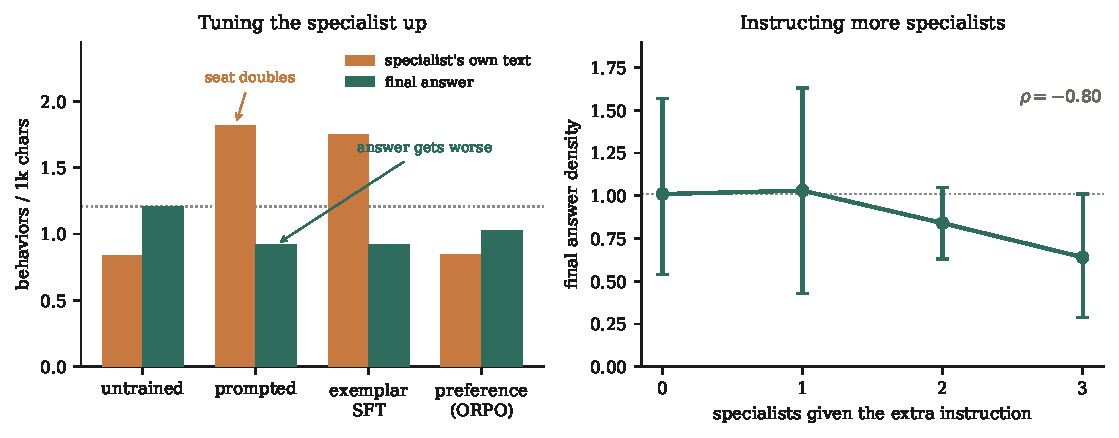
\includegraphics[width=\linewidth]{fig_witness.pdf}
\caption{\emph{Left:} treatments that raise what a specialist writes lower
what the pipeline finally says; the dotted line is the untrained final answer.
\emph{Right:} extending the treatment from zero to three specialists lowers
the final answer monotonically.}
\label{fig:witness}
\end{figure}

\begin{table}[t]
\centering
\caption{The legal specialist under four treatments: what the specialist
writes, and what the pipeline finally says (bootstrap 95\% intervals over
$n=30$ runs each).}
\label{tab:witness}
\begin{tabular}{lcc}
\toprule
Treatment & Specialist's own text & Final answer \\
\midrule
untrained & $0.84$ $[0.62,1.06]$ & $\mathbf{1.21}$ $[0.93,1.49]$ \\
prompted & $\mathbf{1.82}$ $[1.38,2.30]$ & $0.92$ $[0.67,1.19]$ \\
exemplar fine-tuning & $\mathbf{1.75}$ $[1.45,2.08]$ & $0.92$ $[0.72,1.13]$ \\
preference optimization & $0.85$ $[0.58,1.15]$ & $1.03$ $[0.81,1.28]$ \\
\bottomrule
\end{tabular}
\end{table}

Prompting the specialist more than doubles what it writes, from $0.84$ to
$1.82$. Fine-tuning it on qualification-rich examples does the same, $1.75$.
Both are real: the intervals exclude the untrained baseline, and the
specialist's text is visibly more careful. Both make the finished answer
\emph{worse} than leaving the specialist alone---$0.92$ against $1.21$.

Extending the treatment across specialists confirms the direction. Giving the
extra instruction to zero, one, two and then all three specialists produces
final answers of $1.01$, $1.03$, $0.84$, $0.64$: a monotone decline,
$\rho = -0.80$. Care does not accumulate across specialists and then get
diluted. It is not accumulating at all.

The texts suggest why. A specialist told to flag uncertainty everywhere flags
it in every clause, and the result reads less like carefulness than like a
verbal tic. The aggregator, whose instruction asks it to write a clean
integrated answer, treats it accordingly and edits it out. A useful way to
put this: an aggregator is not a channel that passes qualification through
with some loss. It is a writer that decides how much to write, and evidence
of over-qualification upstream is a reason for it to write less.

\section{What specialists actually contribute}
Return to the comparison that matters. A lone prompted model and the full
council are indistinguishable on how much they qualify where qualification is
warranted---$0.50$ against $0.57$. They are not remotely alike on the question
that warrants none. The lone model qualifies it at $0.15$ $[0.08,0.22]$; the
council at $0.00$ $[0.00,0.00]$, on every one of five runs. The intervals are
disjoint.

The reason is in the form of the instruction rather than its content. The
council's aggregator is told, in effect, \emph{if a specialist flagged an
assumption, label it as one; if a specialist flagged that information may have
aged, carry that through}. Every clause is conditional on something a
specialist did. When the specialists flag nothing, the conditions are not met
and nothing fires. The lone model is given the same requirements as standing
instructions, because there is no upstream for them to refer to, so they fire
whether or not anything warrants them. It has learned the form of epistemic
care with none of the judgement: asked a routine question about hybrid-work
communication, it opened with a section headed ``Current State Snapshot (as of
my training data)'' and closed with ``actual results may vary.''

This is what specialists are for. Not to produce more qualification---the
aggregator's instruction sets that, and the specialists barely affect it---but
to produce a record of what was actually uncertain, against which a
conditional instruction can be evaluated. They are witnesses. Their value is
that they can be checked, and it is destroyed if they are trained to say
everything is uncertain, because a witness who always says the same thing
carries no information.

\begin{table}[t]
\centering
\caption{The two effects, separated. ``Volume'' is qualification on questions
that warrant it; ``discrimination'' is its absence on the question that does
not.}
\label{tab:sep}
\begin{tabular}{lcc}
\toprule
Arrangement & Volume & Unwarranted qualification \\
\midrule
one model, no instruction & $0.14$ & $0.00$ \\
three specialists, plain merge & $0.16$ & $0.06$ \\
one model, standing instruction & $0.50$ & $0.15$ \\
three specialists, conditional instruction & $0.57$ & $\mathbf{0.00}$ \\
\bottomrule
\end{tabular}
\end{table}

Table~\ref{tab:sep} makes the decomposition explicit. Volume comes from the
instruction: it is what separates rows three and four from rows one and two.
Discrimination comes from having specialists \emph{and} making the instruction
depend on them: it is what separates row four from row three. Neither
ingredient produces it alone.

\section{Why this cannot be trained in}
The obvious objection is that we simply instructed where we should have
trained. We tried training, at both ends and by three methods, and it does not
work at either.

At the specialist, preference optimization installs no additional
qualification at all---$0.85$ against an untrained $0.84$---and tripling the
training data changes nothing, even though the larger set raised the model's
accuracy at distinguishing good examples from bad from $0.48$ to $0.94$. The
preference was learned and not acted on. Replication on a second specialist of
a different lineage produced no effect; on a third, an effect we had
registered in advance failed to appear.

At the aggregator---the position this paper says decides everything---training
also fails. Fine-tuning it on qualification-rich synthesis examples left its
output where it started, $0.89$ against $1.03$ untrained. We then repeated
this with the reward corrected in every way we could think of: sampling the
aggregator's own outputs rather than a fixed corpus, and scoring them on the
finished answer for qualifying heavily where warranted and not at all where
not. It moved nothing, $0.60$ against $0.56$.

What did survive training is telling. After fine-tuning the aggregator on
precisely the behavior its instructions elicit, the instructions still worked
at full strength---the effect of adding clauses was $1.58\times$ on the
trained model against $1.82\times$ untrained. If instructions and weights were
competing routes to the same behavior, training on that behavior should have
absorbed some of the instruction's job. It did not, which suggests they act on
different things: the weights on what a model tends to do, the instruction on
what it does this time.

We are careful about the strength of this claim. Our training was small---
low-rank adapters over tens of preference pairs, against instruction-following
that model builders installed with vastly more data. ``A small amount of
training did not overwrite a deeply installed capability'' is weaker than
``training cannot do this,'' and it is the one we can support. What we can say
without qualification is that at every scale available to us, the instruction
was free, immediate and effective, and the training was none of those things.

\section{Limitations}
Of five behaviors we set out to count, one fell below detection, so we report
four; the effect of instructions is clear in combination but not for any
single behavior alone. Pattern matching misses paraphrase and rewards brevity;
two further instruments agree with it on the load-bearing comparisons, but all
three are automatic and none is anchored to human judgement.

Everything ran at or below 20B parameters on one machine, with five seeds and
seven questions we wrote ourselves. A frontier model as aggregator could
behave differently, and the question that warrants no qualification carries a
great deal of weight for something measured over five runs. The architecture
comparison uses one model family in every role and one implementation of each
design.

We also report defects in our own record rather than repairing them. One model
we intended as a comparison produced degenerate output---26 of 30 answers were
fragments ending mid-sentence---which we found only after computing a figure
from them; that arm is withdrawn, and with it a comparison between alignment
lineages we had intended to make. In our earliest arms, five runs per question
are in fact one run from an earlier session plus four from a later one, and
133 runs record a batch label where a model identifier belongs. None of this
changes a reported interval, but it weakens those arms' internal consistency.

\section{Conclusion}
Specialist agents in a pipeline are usually justified by what they know and
defended by how carefully they say it. Neither holds up here. A
domain-specialised model is no more epistemically careful than a generic one
of similar size until it is told to be, and once several of them are told to
be, the finished answer gets worse rather than better. A single well-prompted
model matches a full council for how much it qualifies.

But the council was the only arrangement that knew when to stop, and that is
not a small thing---it is the difference between a system whose caution means
something and one that hedges reflexively. It came from an instruction that
could check what the specialists had actually flagged, which is the one thing
a solitary model cannot do at any level of prompting.

So the role specialists play is real but narrow. They are witnesses. What they
are for is being checkable, and the way to ruin them is to train them to
qualify everything, because a witness who always says the same thing tells you
nothing. Build them to flag what is genuinely uncertain and no more. Put the
effort into the aggregator's instruction, make every clause of it conditional
on what the specialists said, and stop fine-tuning components for epistemic
quality, which in our hands never reached the page.

\paragraph{Reproducibility.} Code, prompts, all runs, pre-registrations,
protocol amendments, refuted predictions, and an integrity audit that withdrew
one arm: \url{https://github.com/srbobo/council-of-experts-research}.

\appendix

\section{The aggregator's instruction}
\label{app:prompt}
The aggregator writes in two steps---first identify tensions between the
specialists, then write the integrated answer. The second step carries five
requirements, of which three are the preservation clauses. Verbatim:

\begin{quote}\small
\textbf{1.} Acknowledge the tensions you just identified---not abstractly, but
at the points where they bite the answer.

\textbf{2. PRESERVE numeric framing}---if a specialist labeled a number as a
modeled assumption, your synthesis MUST also label it as an assumption (use
``modeled at,'' ``assumed''). Never adopt a specialist's modeled number as a
fact.

\textbf{3. PRESERVE precise vocabulary}---if a specialist used a specific legal
term, jurisdiction, FDA pathway, or clinical concept, preserve it; do not
smooth out precision in the name of accessibility.

\textbf{4. PRESERVE caveats}---if a specialist flagged training-cutoff
uncertainty or data fragility, propagate that flag into your synthesis.

\textbf{5.} Use whatever structure best fits the user's question.
\end{quote}

Clauses 2--4 are conditional on something a specialist did; clause 1 is not,
and when tested alone it changes nothing. Isolating the clauses shows each
lifting the behavior it names and no other, which is why we describe them as
specifications rather than as general encouragement to be careful.

\section{Instruments}
\label{app:instr}
Pattern matching over four behavior families is the primary measure. Two
independent instruments check the load-bearing comparisons: an entailment
model calibrated against our own construction-labelled pairs, and blinded
pairwise LLM judges shown both texts in each order and required to quote the
evidence for their verdict. Where all three agree we report the result; where
they disagree we report the disagreement. One finding did not survive---an
apparent \emph{increase} in hedging on the finance specialist appeared under
pattern matching alone, and neither other instrument saw it. We retired it as
an artifact of the measure.

\end{document}
